\subsection*{ViT-V-Net: Vision Transformer for Unsupervised Volumetric Medical Image Registration}

% \subsection*{Ссылка} \url{https://arxiv.org/abs/2104.06468}
\subsubsection*{Введение}
Несмотря на хорошую производительность, сверточные нейронные сети
в общем случае имеют  ограничения в моделировании явных
пространственных отношений на большом расстоянии (например, 
отношения между двумя вокселями, которые находятся далеко друг от друга), 
присутствующих в изображении из-за локальности операции свертки.
Для преодоления этого ограничения были предложены различные решения, такие как 
U-Net \cite{Unet}, atrous convolution и self-attention. Недавно возрос интерес 
в проектировании архитектуры, основанной на самовнимании (self-attention), 
которая хорошо проявила себя в обработке естественного языка. Была 
предложена ViT - архитектура, целиком и полностью основанная на self-attention.
В данной работе исследуется применение ViT в объемных медицинских изображениях.
Авторы предлагают ViT-V-Net \cite{VitVNet}, которая воплощает в себе гибридную архитектуру
\glqq сверточная нейронная сеть \cite{VNet}-трансформер\grqq (ConvNet-Transformer) для применения self-supervised 
метода в исследовании трехмерных медицинских изображений.
\subsubsection*{Основная идея}
В предложенном методе ViT \cite{Transformers} была применена к высокоуровневым признакам изображений, что
требовало от сети выявить зависимости между точками, находящимися на дальнем расстоянии.
Наивное применение ViT к полномасштабным изображениям приводит к увеличению вычислительной 
сложности. Поэтому, изображения сначала были закодированы с помощью
нескольких сверточных слоев и слоев max-pooling для получения объектов,
содержащих высокоуровневые признаки. Далее, в ViT, высокоуровневые признаки делятся на патчи, 
а затем патчи отображаются в скрытое пространство с помощью обучаемой 
линейной проекции (например, patch embedding). Затем, результирующие патчи 
подаются в энкодер трансформера, а полученный выход декодируется V-Net подобным декодером. 
\\
\begin{minipage}{1.0\linewidth}
    \begin{center}
        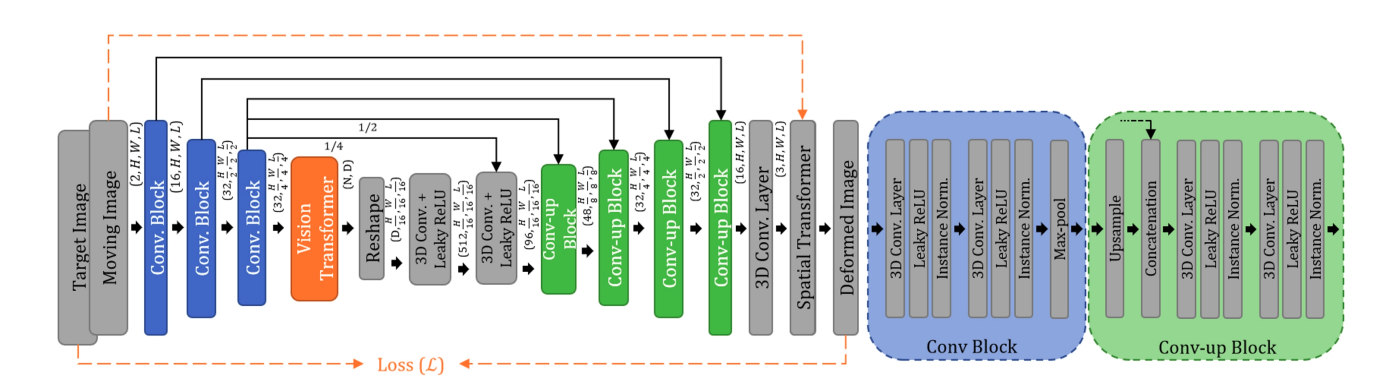
\includegraphics[scale=0.3]{ann12-arch.png} \\
        \captionof{figure}{\scriptsize{Архитектура ViT-V-Net.}}
    \end{center}
    
\end{minipage}
\subsubsection*{Данные}
МРТ-изображения в модальности Т1-ВИ.
\subsection*{Результаты}
Был проведен сравнительный анализ предложенного метода с методами Symmetric 
Normalization (SyN), NiftyReg и VoxelMorph-1 и -2 по мере Серенсена (Dice score).
В результате ViT-V-Net более превзошла более, чем на 0.1 все рассматриваемые методы.
\\
\begin{minipage}{1.0\linewidth}
    \begin{center}
        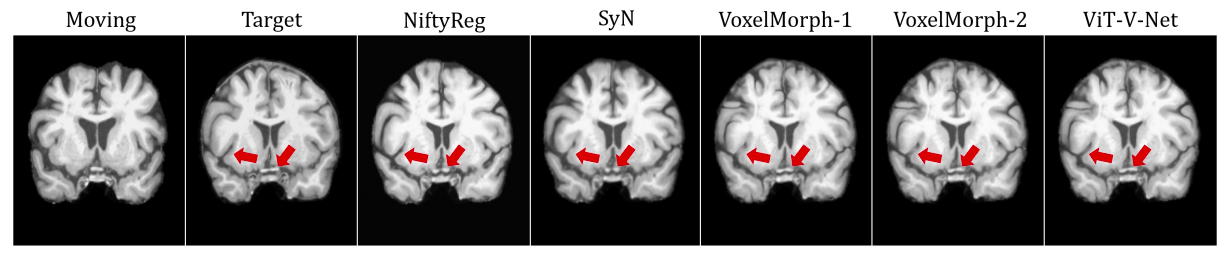
\includegraphics[scale=0.3]{ann12-mri-res.png} \\
        \captionof{figure}{\scriptsize{Результаты предсказания на корональном срезе МРТ.}}
    \end{center}

\end{minipage}

\subsubsection*{Заключение}
Предложенная архитектура, основанная на ViT достигла большей производительности, чем 
существующие методы и показала свою эффективность.